\subsection{Graph}
%Ein Graph G besteht aus einer nichtleeren Menge an Knoten V und Kanten E.
%Ein Graph ist mathematisch folgendermaßen definiert:
Die Grundlage aller Graphdatenbankmodelle liefert die Definition eines einfachen Graphen:
\begin{definition}
	Ein $\text{Graph } G=(V,E,\gamma)$ ist ein Tripel bestehend aus:
	\begin{itemize}
		\item $V$, einer nicht leeren, ungeordneten Menge von Knoten (vertices)
		\item $E$, einer Menge von Kanten (edges)
		\item $\gamma$ , einer Inzidenzabbildung (incidence relation), mit\\
		$\gamma : E \longrightarrow \{X | X \subseteq V, 1 \leq |X| \leq 2\}$
	\end{itemize}\cite[Seite 21]{pbeck01}
%	Ein Knoten $a \in V$ und eine Kante $e \in E$ heißen inzident (incident)
%	genau dann wenn $a$ entweder Anfangs- oder Endecke von $e$ ist. Es gilt $a \in \gamma(e)$.
%	Zwei Knoten $a,b \in V$ heißen adjazent(adjacent) genau dann wenn es eine Kante $e$ gibt die zu $a$ und $b$ inzident ist.
%	Es gilt	$\exists e \in E: \gamma(e)=\{a,b\}$.
\end{definition}
Ein Knoten repräsentiert ein Element in einem Graphen und die Kanten stellen die Beziehung zwischen den einzelnen Knoten her.
%In einem einfachen Graphen kann eine Kante immer nur jeweils zwei Knoten miteinander verbinden.
Bei einfachen Graphen können die Kanten nur die Kardinalität $1 \leq |X| \leq 2$ haben.
Als Kardinalität wird die Anzahl Knoten bezeichnet, die durch eine Kante in Beziehung gesetzt werden kann.
Zwei Knoten heißen adjazent, wenn diese über eine Kante direkt miteinander verbunden sind.
Eine Kante die mit einem Knoten verbunden ist wird als inzident zu diesem Knoten bezeichnet \cite{knauer2015diskrete}.

%\subsection{Eigenschaften von Kanten}
Graphen können gerichtet oder ungerichtet sein.
Gerichtete Graphen zeichnen sich dardurch aus, dass die Kanten eine zugewiesene Richtung besitzen.
Grafisch werden gerichtete Kanten in der Regel durch Pfeile dargestellt.
Für die Modellierung von realen Gegebenheiten ist das Konzept der gerichteten Graphen sehr entscheidend, da dieses die Darstellung einseitiger Beziehungen zwischen den Entitäten des Modells erlaubt.

Um die Beziehung zwischen zwei Knoten genauer zu definieren, lassen sich die Kanten gewichten.
Dabei werden den Kanten in der Regel nummerische Werte zugeordnet und man bezeichnet diese Graphen als gewichtete Graphen.
Durch die Wichtung von Kanten lassen sich beispielsweise Kosten oder Distanzen zwischen den Entitäten definieren.

Ein Knoten ist isoliert, wenn er keine inzidenten Kanten und somit keine direkten Nachbarn hat \cite{knauer2015diskrete}.
Ein ungerichteter Graph heißt zusammenhängend, falls es zwischen zwei beliebigen Knoten $a$ und $b$ aus $V$ einen ungerichteten Weg mit $a$ als Startknoten und $b$ als Endknoten gibt \cite[36-38]{krumke2012graphentheoretische}.
Hat eine Kante als Start- und Endknoten den selben Knoten, verbindet also den Knoten mit sich selber, spricht man von einer Schlinge.
Liegen zwischen zwei Knoten eines Graphen mehr als eine Kante, nennt man diese Multikante.
Enthält ein Graph Multikanten und Schlingen ist dies kein einfacher Graph mehr sondern ein Multigraph \cite{felsner01}.
%Schlingen und Multikanten dürfen in einem einfachen Graphen nicht auftauchen.\cite{felsner01}

Der Grad eines Knoten bezeichnet die Anzahl der inzidenten Kanten des Knoten.
Dabei werden Schleifen doppelt gezählt \cite{rahm2017}.
Ein Graph, bei dem alle Knoten den selben Knotengrad haben, wird als regulärer Graph bezeichnet \cite{felsner2012geometric}.
%Abbildung \ref{2.regular.image} zeigt einen regulären Graphen mit Knotengrad null und einen mit einem Grad von drei.
%\begin{center}
%	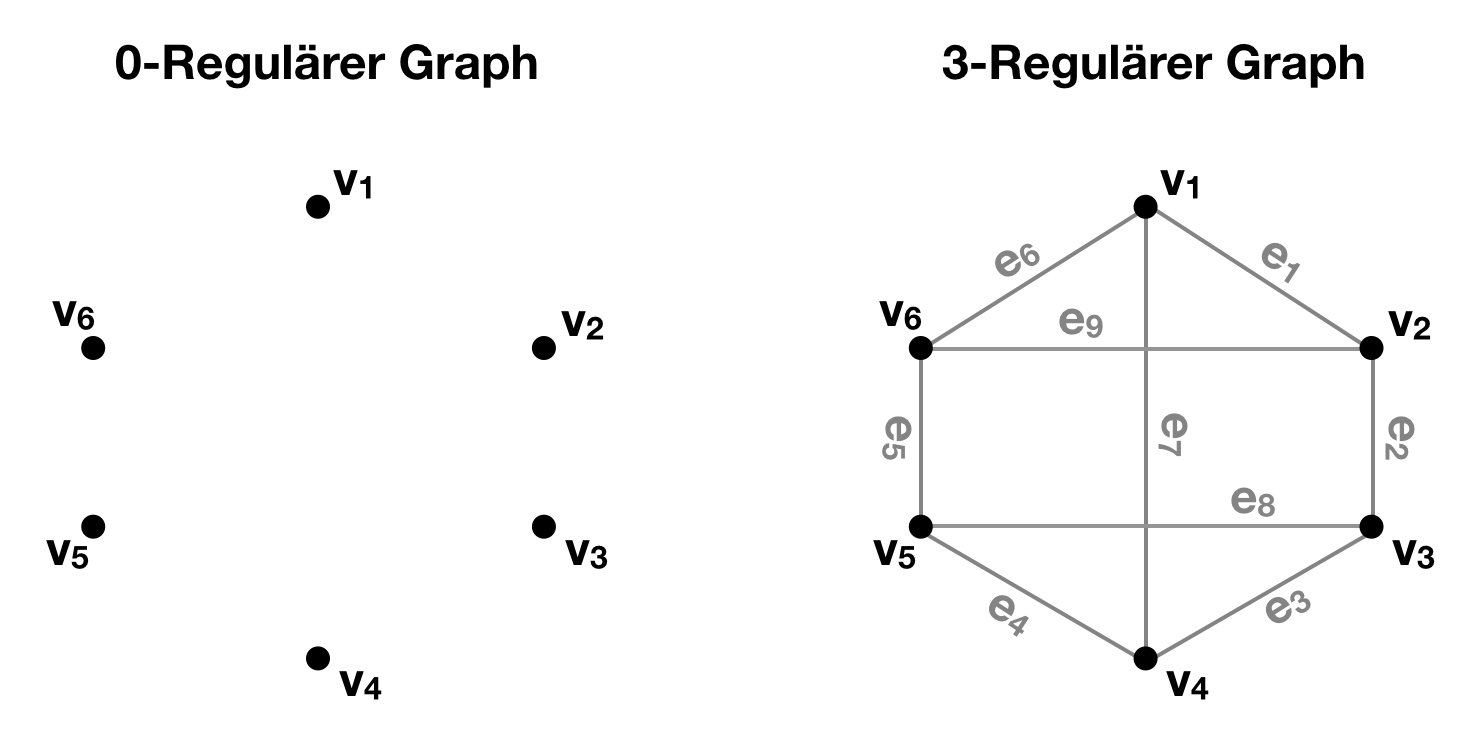
\includegraphics[scale = 0.4]{./images/Regulaerer_graph.png}
%	\label{2.regular.image}
	%\caption{Regulärer Graph}
%\end{center}
Sind bei einem Graphen alle Knoten mit allen übrigen Knoten verbunden, spricht man von einem vollständigen Graphen:
\[K_{n}=\big([n],\begin{pmatrix}
					 [n] \\ 2
\end{pmatrix}\big)\]

%Werden Kanten und Knoten eines Graphs vertauscht, entsteht der Kantengraph bzw. Line-Graph des jeweiligen Graphen L(G).
Da bei einem Graphen nur die Struktur definiert ist, also welcher Knoten über welche Kante mit den anderen Knoten verbunden ist, können Graphen auf unterschiedliche Weisen gezeichnet werden und trotzdem gleich sein.
Sind zwei Graphen gleich, bezeichnet man diese als isomorph \cite[Seite 22]{basicgraphtheory}.
%
%Das simpelste Graphdatenbankmodell ist ein einfacher gelabelter Graph.
%
%Subgraphen
%\subsection{Reguläre Graphen}
%Bei regulären Graphen haben alle Knoten den selben Knotengrad.
%Als Knotengrad wird die Anzahl direkter Nachbarn, also alle Knoten die über eine Kante direkt mit dem betrachteten Knoten verbunden sind, bezeichnet.\cite{felsner2012geometric}
%Abbildung \ref{2.regular.image} zeigt einen regulären Graphen mit Knotengrad null und einen mit einem Grad von drei.
%\begin{center}
%	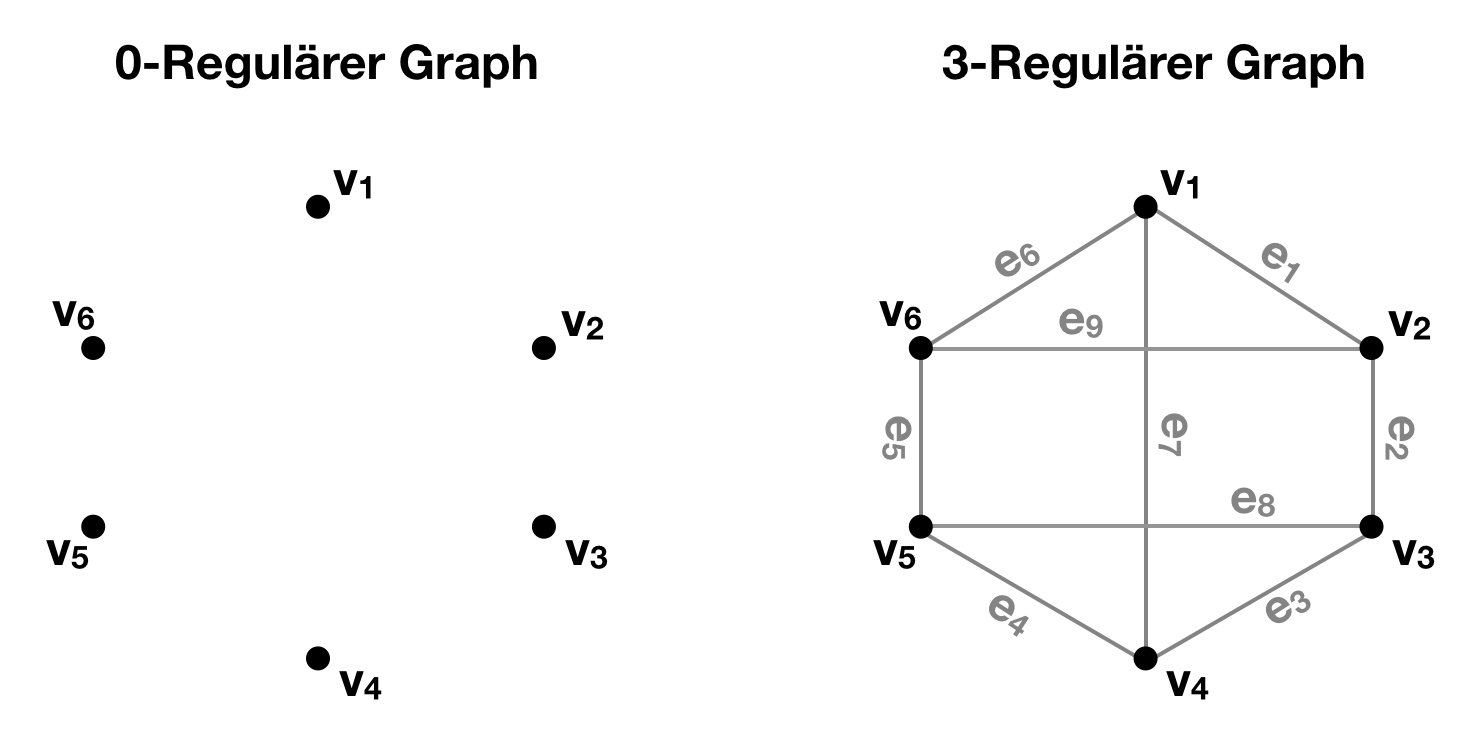
\includegraphics[scale = 0.4]{./images/Regulaerer_graph.png}
%	\label{2.regular.image}
%	%\caption{Regulärer Graph}
%\end{center}